% Document settings

% Common
\DocumentMetadata{pdfversion=1.7, pdfstandard=A-2u}
\documentclass[11pt,letterpaper]{article}
\usepackage{fancyhdr}
\usepackage[]{fncychap}
\usepackage{etoolbox} % patch stuff
\usepackage[margin=1in]{geometry}
\usepackage{multirow}
\usepackage{longtable,booktabs, array, threeparttable} % typesetting
\usepackage{bookmark}
\usepackage[acronym]{glossaries-extra}
\pagestyle{plain}
\usepackage{parskip, setspace}

% Plots and Color
\usepackage{graphicx}
\graphicspath{{images/}{drawings/}}
\usepackage[font=footnotesize,labelfont=bf]{caption}
\usepackage{xcolor,colorspace}
\usepackage{tcolorbox}
\usepackage{pgfplots}
\pgfplotsset{compat=newest}
\usepackage{epstopdf}
\usepackage[american voltages]{circuitikz}


% Math stuff
\usepackage{mathtools} % loads amsmath and fixes its bugs, empheq, etc
\usepackage{amssymb}
\usepackage{sympytex}
\usepackage{siunitx}
\sisetup{detect-all=true}   % ensure proper font weight
\sisetup{per-mode = repeated-symbol}    % ensure "/" unit delineator
\sisetup{range-phrase = {\text{~to~}}}  % SI range clarity (NIST 811 Ch7.7)
\DeclareMathSymbol{\varOmega}{\mathalpha}{operators}{"0A}   % upright omega for ohms
\providecommand*{\Ohm}{\varOmega}   % for siunitx
\DeclareSIUnit\sq{\ensuremath{\Box}}    % sheet resistance
\DeclareSIUnit{\Siemens}{S}
\DeclareSIUnit{\torr}{Torr} % add torr to siunitix 3
\DeclareSIUnit\sig{\ensuremath{\sigma}}
\DeclareSIUnit\ppm{ppm}
\usepackage{xfrac}

% Font
\usepackage{fontspec}
\setmainfont{STIXTwoText}[
	Extension		= .otf,
	UprightFont		= *-Medium,
	BoldFont		= *-Bold.otf,
	ItalicFont		= *-MediumItalic.otf,
	BoldItalicFont 	= *-BoldItalic.otf
]
\usepackage[warnings-off={mathtools-colon,mathtools-overbracket},math-style=ISO]{unicode-math}
\setmathfont{STIXTwoMath-Regular.otf} % for symbols
% \usepackage{microtype}
% \UseMicrotypeSet[protrusion]{basicmath} % disable protrusion for tt fonts
\urlstyle{same}

\usepackage[normalem]{ulem} % Enable normal \ul underline
\usepackage{fancyvrb}

\RequirePackage[type={CC},modifier={by-nc-nd},version={4.0},lang={english}]{doclicense}

\usepackage{datetime2} % to satisfy the "\today" in \hypersetup
\DTMusemodule{english}{en-US}
\usepackage{hyperref}
\hypersetup{
    hyperindex=true,
    colorlinks=true,
	bookmarksnumbered,
    bookmarksopen=true,
    linkcolor=blue,
    filecolor=magenta,      
    urlcolor=cyan,
%%%%%%%%%%%%%%%% METADATA %%%%%%%%%%%%%%%%%%%%	
    pdftitle={EE726 Project 3},
	pdfsubject={4-Bit StrongARM Flash ADC},
    pdfauthor={Chris Biancone},
	pdfpublisher={Chris Biancone},
	pdfkeywords={rail-to-rail; StrongARM; flash ADC},
%%%%%%%%%%%%%%%%%%%%%%%%%%%%%%%%%%%%%%%%%%%%%%
	pdfproducer=luaLaTeX-1.17.0,
	pdfdate=\today,
	pdflang={en},pdfmetalang={en},
	pdflicenseurl={},
    % pdfpagemode=FullScreen,
}
\usepackage[nameinlink,capitalize]{cleveref}
% this is necessary for IEEEtranDOI.bst to work with hyperkinked DOIs
\newcommand*{\doi}{}
\makeatletter
\newcommand{\doi@}[1]{\href{https://doi.org/#1}{#1}}
\DeclareRobustCommand{\doi}{\hyper@normalise\doi@}
\makeatother

% % % % % % % % % % % Header footer
% % % % % % % % % % %EDIT THIS % % % % % % % % % % % % % % % % % % % %
\pagestyle{fancy}
\fancyhf{}
\lhead{Tech Memo:  Project 3}
\rhead{Chris Biancone}
\lfoot{EE726}
\cfoot{\today }
\rfoot{Page \thepage}
% % % % % % % % % % % % % % % % % % % % % % % % % % % % % % % % % % % % %

% Scale images if necessary, so that they will not overflow the page
% margins by default, and it is still possible to overwrite the defaults
% using explicit options in \includegraphics[width, height, ...]{}
%\setkeys{Gin}{width=\maxwidth,height=\maxheight,keepaspectratio}

% No paragraph indent
\setlength\parindent{0pt}

\begin{document}

\VerbatimFootnotes % allows verbatim text in footnotes

\numberwithin{equation}{subsection}
\numberwithin{figure}{subsection}

	\hspace{4.5in}
	
\includegraphics[width=2in,trim=0cm 0in 0in 0.0in,clip]{kgcoelogo2019horiz.eps}
\newline

\Huge\textbf{EEEE 726: Project 3 \\4-Bit StrongARM Flash ADC}\\

\Large
\textbf{From:} Chris Biancone \\
\textbf{To: } Dr. Mark Pude \\
\textbf{Date: } 04/02/2024 \\
\textbf{Subject: } Project 3\\
\vspace{0.5in}

\section*{Abstract}
\normalsize
The purpose of this project is to design a flash ADC incorporating the previously designed comparator. The RTR StrongARM-based comparator is refined to enhance the performance in this application. A 4-bit design is chosen based on the requirement for <\qty{25}{\dB} SQNR and each binary output is designed to drive a \qty{1}{\pF} capacitive load. This ADC has been tested to work in a rail-to-rail configuration with a reference voltage of \qty{2}{\V}, equal to the nominal supply voltage. In schematic-level simulations, a DNL of \qty{20.848}{mLSB}, INL of \qty{1.2009}{mLSB}, and propagation delay of \qty{2.7531}{\ns} are achieved at \(V_{LSB_{eff}}\) = \qty{133}{\mV}.

\section{Design}

\subsection{SQNR}

It is known that SQNR in an ADC system is a function of the bit depth of the ADC, since quantization noise is determined by the effective \(V_{LSB}\), shown in \cref{eq:sqnr}.

\begin{align}
    \mathrm{SQNR} &= 20\log\biggl(\frac{V_{in,rms}}{V_{Q,rms}}\biggr) \quad , \quad V_{Q,rms} \triangleq \frac{V_{LSB}}{\sqrt[]{12}}\\
    \mathrm{SQNR} &\approx 6.02\,N + \qty{1.76}{\dB}\label{eq:sqnr}
\end{align}

Thus, selecting \(N\) = 4 yields an SQNR = \qty{25.84}{\dB}, satisfying the design requirement of \qty{25}{\dB}. While this figure has little margin, SQNR is only a function of fundamental design aspects of the ADC as shown and will not vary with environmental conditions like noise or even reference voltage ranges.

\subsection{Top-Level}

A standard resistor ladder was adopted for this ADC design to divide the reference voltage into individual references for each comparator's negative input. The resistors are arranged in an R : 2R $\cdots$ 2R : R configuration from top to bottom to divide the range into 2\textsuperscript{\emph{N}} ranges with 2\textsuperscript{\emph{N}}-1 voltages. The values of these resistors are selected to be \qty{13}{\kilo$\Omega$}, which provides a balance of minimizing current draw from this stage and maintaining a reduced time constant when in parallel with input capacitances of the comparators. This is necessary for kickback noise that appears from the latched comparators to settle before their next sample. If the kickback voltage is significant compared to the voltage for each code, this can result in glitches in the output. \cref{Fig:flash} shows the full top-level schematic of the flash ADC, which consists mainly of the resistor network, comparators, and a thermometer-to-binary encoder for digitizing the comparator outputs. The resistor network shows 2 parallel resistors for matching purposes and dummy resistors provided on the sides for yield in manufacturing.

 \begin{figure}[htbp!]
		\centering
		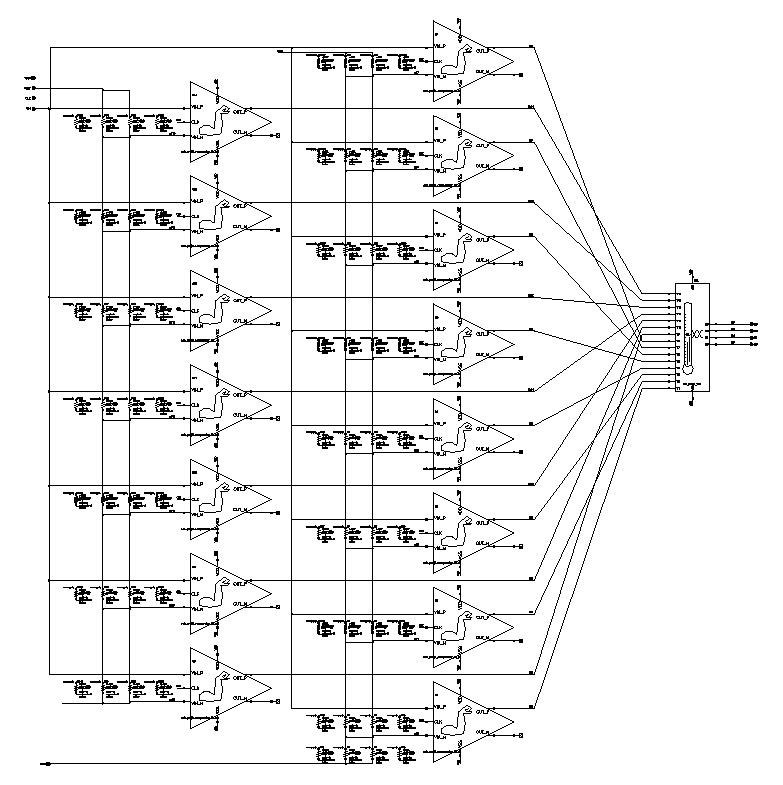
\includegraphics[width=4in]{flash_old.eps}
		\caption{Top-level schematic of the flash ADC.}\label{Fig:flash}
	\end{figure}

The StrongARM comparator employed in this ADC is designed to process rail-to-rail common mode signals, allowing the same exact comparator design to be used for every position. This avoids any mismatch in input capacitance and should contribute toward gain linearity across the common mode range.

\subsection{Encoder}

Some form of encoder subsystem is necessary in the flash ADC to translate the ``thermometer''-coded output of the 15 comparators into 4-bit binary. Various methods have been explored in industry and literature, including Wallace tree, Fat-tree, ROM, and MUX based designs. A MUX-based encoder design based on~\cite{Lee2013} is used for its low-power operation and high speed at the cost of high device count, shown in \cref{Fig:encoder}. Additional power savings and reduction in the number of required devices is provided through the use of transmission gate-based MUXs shown in \cref{Fig:tgmux2}, which use half the number of devices as active CMOS multiplexers. Due to the load that the transmission gates put onto the comparators and to provide some delay time correction, the binary signals are sent through a network of inverters and buffers to provide MUX control logic and the eventual outputs, which are sized as shown in \cref{Fig:buf}.

\begin{figure}[htbp!]
    \centering
    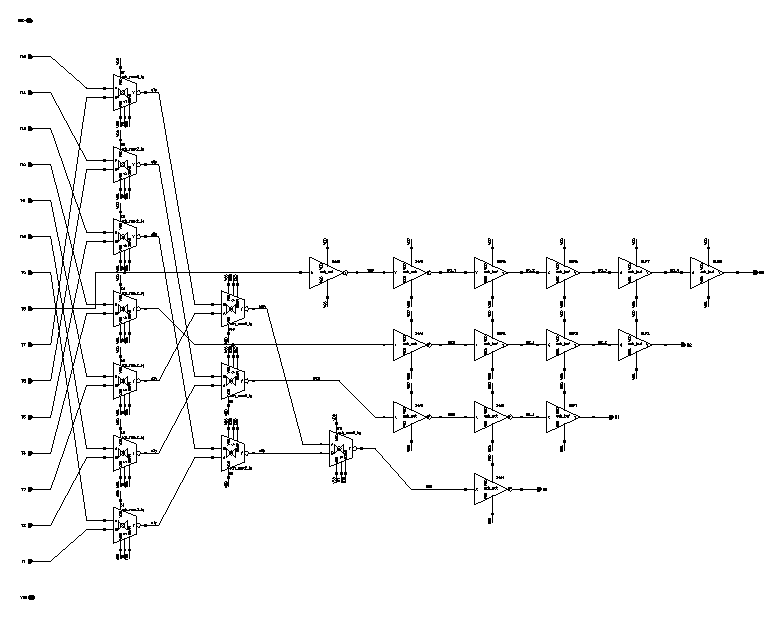
\includegraphics[width=4in]{encoder_old.eps}
    \caption{Schematic view of encoder design.}\label{Fig:encoder}
\end{figure}

\begin{figure}[htbp!]
    \centering
    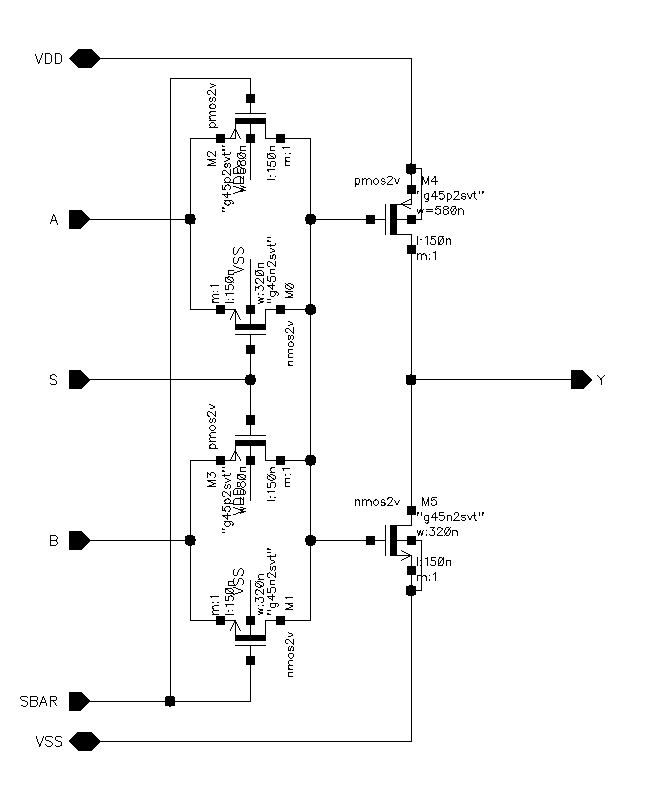
\includegraphics[width=3in]{tgmux2.eps}
    \caption{Schematic of transmission-gate based MUX that provides the functionality of the proposed encoder design. The outputs are inverted for logic purposes and increased drive strength.}\label{Fig:tgmux2}
\end{figure}

\begin{figure}[htbp!]
    \centering
    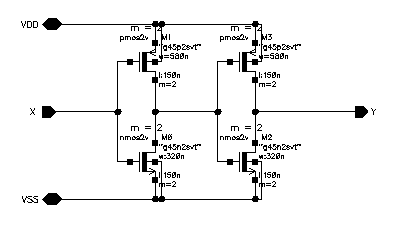
\includegraphics[width=4in]{buf.eps}
    \caption{Schematic of buffer highlighting device sizes, which are also used in the inverter design.}\label{Fig:buf}
\end{figure}


\section{Schematic Level Simulations}

Preliminary schematic level simulations have been run at typical corner of \qty{27}{\degree\C} and \qty{2}{\V} \(V_{DD}\). The schematic was captured and simulated using C\=adence Virtuoso. 

Currently, using SPECTRE APS with ++aps and +mt=8 at conservative error preset, setting \(GND\), \(V_{DD}\), and \(V_{ref}\) nodes to their values, and setting IC=0 on appropriate internal nets, running 1 test takes \~4:\qty{15}{min} at 10 clocks per code. Increasing to a more appropriate 100 clocks per code for \qty{0.01}{LSB} resolution of INL and DNL increases simulation time to around \qty{20}{min}. Various measures to decrease the simulation time are being investigated to capture appropriate PVT corner and monte carlo data in a reasonable time.

\subsection{INL and DNL Testbench}

A simple testbench schematic was set up for the flash ADC as shown in \cref{fig:tb-sch}. The local ground for this design is decoupled from the global ground using a \qty{0}{\V} source, and currently a VCVS is used to increase the given reference voltage of \qty{1}{\V} up to \qty{2}{\V} for testing rail-to-rail operation. In a full system, a reference voltage at the power supply would likely need to be supplied by an LDO and possibly assisted by a charge pump. The supplied \qty{12}{\MHz} clock is realized by a pulse source with 5\% rise and fall times, and the input triangle ramp is supplied by a piecewise-linear source. This is defined based on the clock period and is paramatrized along with the simulation time, so that the number of samples per code can be chosen.

Each output bit from the encoder drives a \qty{1}{\pF} load as specified, and are also sent into an ideal 8-bit DAC provided by the \emph{ahdlLib}. This DAC is intended to translate the binary ADC output into a stepped ramp output for comparison with the ideal stepped ramp output with idealized trip voltages. Once normalized for any gain and offset error using the first and last transitions to find a \(V_{LSB_{eff}}\), the difference in code widths for the output of the ADC compared to the ideal version allows for quantification of differential nonlinearity (DNL). The summation of these differences across the range provides the integral nonlinearity (INL).

\begin{figure}[!t]
    \centering
    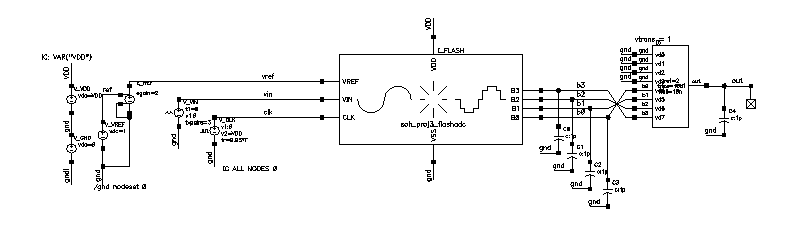
\includegraphics[width=6in]{flash_tb_old.eps}
    \caption{Testbench setup used for INL and DNL analysis.}
    \label{fig:tb-sch}
\end{figure}

The achieved results for INL and DNL at typical corner are shown in \cref{fig:inldnl}. \(V_{LSB_{eff}}\) was calculated to be \qty{133}{\mV}.

\begin{figure}[htbp!]
    \centering
    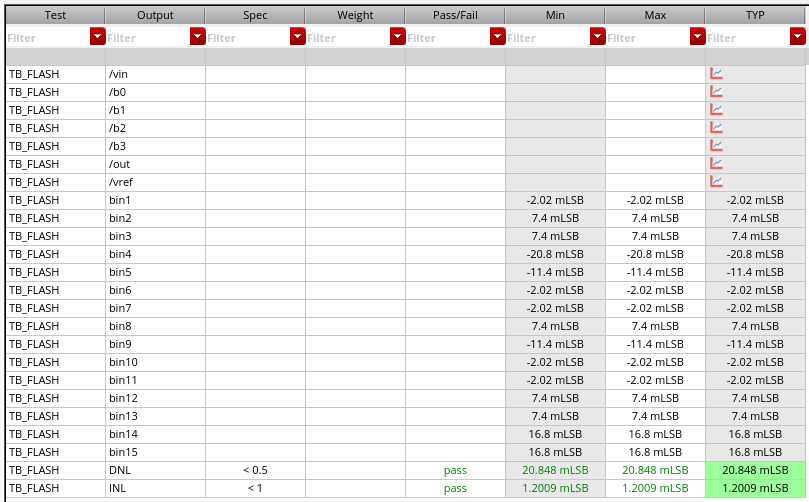
\includegraphics[width=4in]{INL_DNL_TYP_old.png}
    \caption{INL and DNL results at typical.}
    \label{fig:prop-plot}
\end{figure}

\subsection{Propagation Delay Testbench}

To analyze propagation delay, the same testbench setup was used but with a modified PWL input to step nearly instantaneously right before each clock rise. This was intended to have all of the comparators slam high at once, and the last output bit to fall into place was measured for propagation delay. The results are shown in \cref{prop}

\begin{figure}[htbp!]
    \centering
    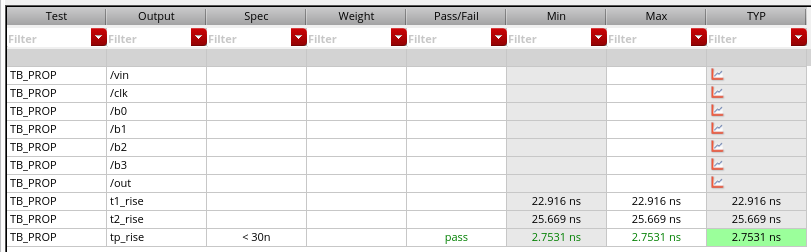
\includegraphics[width=4in]{TP_TYP_old.png}
    \caption{Propagation delay results at typical.}
    \label{fig:prop}
\end{figure}


\subsection{Results}


\section{Layout}

Revised layout of the comparator is completed, along with layout for each of the individual blocks within each of the schematics shown above. Since redoing the comparator layout, it has been tested to run in extracted simulations at \qty{1.1}{\GHz} with <\qty{20}{\mV} hysteresis.

\section{Extracted Results}


\section{Conclusion}


\newpage

\bibliographystyle{bib/IEEEtranDOI}
\bibliography{bib/main.bib}

\end{document}